\documentclass[12pt]{article}
\usepackage[utf8]{inputenc}
\usepackage{float}
\usepackage{amsmath}
\usepackage{amsthm}

\usepackage[hmargin=3cm,vmargin=6.0cm]{geometry}
%\topmargin=0cm
\topmargin=-2cm
\addtolength{\textheight}{6.5cm}
\addtolength{\textwidth}{2.0cm}
%\setlength{\leftmargin}{-5cm}
\setlength{\oddsidemargin}{0.0cm}
\setlength{\evensidemargin}{0.0cm}

%misc libraries goes here
\usepackage{tikz}
\usepackage{tikz-qtree}
\usetikzlibrary{automata,positioning}

\begin{document}

\section*{Student Information} 
%Write your full name and id number between the colon and newline
%Put one empty space character after colon and before newline
Full Name :  Onur Can TIRTIR\\
Id Number :  2099380\\

% Write your answers below the section tags
\section*{Answer 1}

\subsection*{a.}

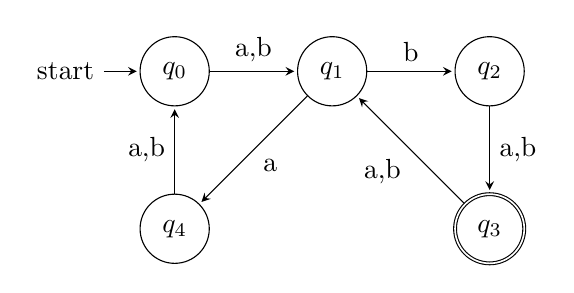
\begin{tikzpicture}
    [>= stealth, shorten >= 1pt,node distance = 2cm,on grid,auto]
\node[state,initial](0){$q_0$};
\node[state](1)[right = of 0]{$q_1$};
\node[state](2)[right = of 1]{$q_2$};
\node[state](4)[below left = 2 cm and 2 cm  of 1]{$q_4$};
\node[state,accepting](3)[below = of 2]{$q_3$};

\path[->]
    (0) edge node {a,b} (1)
    (1) edge node {b} (2)
    (1) edge node {a} (4)
    (4) edge node {a,b} (0)
    (3) edge node {a,b} (1)
    (2) edge node {a,b} (3);
\end{tikzpicture}

$M=\{\{q_0, q_1, q_2, q_3, q_4\}, \{a, b\}, \delta, q_0, \{q_3\}\}$ where,
\begin{flalign*}
    & \delta(q_0, a) = q_1 & \\
    & \delta(q_0, b) = q_1 & \\
    & \delta(q_1, a) = q_4 & \\
    & \delta(q_1, b) = q_2 & \\
    & \delta(q_2, a) = q_3 & \\
    & \delta(q_2, b) = q_3 & \\
    & \delta(q_3, a) = q_1 & \\
    & \delta(q_3, b) = q_1 & \\
    & \delta(q_4, a) = q_0 & \\
    & \delta(q_4, b) = q_0 & \\
\end{flalign*}

Applying partitioning procedure for states, initially we have two partitions, $A_1=\{q_3\}$ and $A_2=\{q_0, q_1, q_2, q_4\}$. \\
$(q_0, a, q_1\in A_2),(q_0, b, q_1\in A_2),(q_1, a, q_4\in A_2),(q_1, b, q_2\in A_2)\in M$. Hence $q_0$ and $q_1$ can be in the same partition. \\
$(q_1, a, q_4\in A_2), (q_2, a, q_3\in A_1)\in M$. Hence $q_1$ and $q_2$ cannot be in the same partition. \\
$(q_2, a, q_3\in A_1), (q_4, a, q_0\in A_2)\in M$. $q_2$ and $q_4$ they cannot be in the same partition. \\
$(q_0, a, q_1\in A_2),(q_0, b, q_1\in A_2),(q_4, a, q_0\in A_2),(q_4, b, q_0\in A_2)\in M$ in the automaton. Hence $q_0$ and $q_4$ can be in the same partition. \\

Now we have three possible partitions $A_1=\{q_0, q_1, q_4\}$, $A_2=\{q_2\}$ and $A_3=\{q_3\}$.\\
$(q_0, b, q_1\in A_1), (q_1, b, q_2\in A_2)\in M$. Hence $q_0$ and $q_2$ cannot be in the same partition. \\
$(q_1, b, q_2\in A_2), (q_4, b, q_0\in A_1)\in M$. Hence $q_1$ and $q_4$ cannot be in the same partition. \\
$(q_0, a, q_1\in A_1),(q_0, b, q_1\in A_1),(q_4, a, q_0\in A_1),(q_4, b, q_0\in A_1) \in M$. Hence $q_0$ and $q_1$ can be in the same partition. \\

Now we have four possible partitions $A_1=\{q_0, q_4\}$, $A_2=\{q_2\}$, $A_3=\{q_3\}$ and $A_4=\{q_1\}$.\\
$(q_0, b, q_1\in A_4), (q_4, b, q_0\in A_1)\in M$. Hence $q_0$ and $q_2$ cannot be in the same partition. \\

So it can be said that we already have the minimal number of states in our automaton.

\subsection*{b.}

\begin{flalign*}
%E_{q_0} & = (a\cup b)\Big(b(a\cup b)(a\cup b)\Big)^*a(a\cup b)^* \\
%E_{q_1} & = (a\cup b)\Big(a(a\cup b)(a\cup b) \cup b(a\cup b)(a\cup b)\Big)^* \\
%        & = (a\cup b)\Big((a\cup b)(a\cup b)(a\cup b)\Big)^*
%
%E_{q_0} & = \Big((a\cup b)a(a\cup b)\Big)^* \cup  L(a\cup b)a(a\cup b)  & \\
%E_{q_1} & = (a\cup b)\Big(a(a\cup b)(a\cup b)\Big)^* \cup L(a\cup b)    & \\
%E_{q_2} & = L(a\cup b)b \cup (a\cup b)\Big(a(a\cup b)(a\cup b)\Big)^* b & \\
%E_{q_3} & = L                                                           & \\
%E_{q_4} & = L(a\cup b)a \cup (a\cup b)a\Big((a\cup b)(a\cup b)a\Big)^*  & \\ \\
    E_{q_0} & = \Big(\Sigma a\Sigma\Big)^* \cup  L\Sigma a\Sigma  & \\
    E_{q_1} & = \Sigma\Big(a\Sigma\Sigma\Big)^* \cup L\Sigma    & \\
    E_{q_2} & = L\Sigma b \cup \Sigma\Big(a\Sigma\Sigma\Big)^* b & \\
    E_{q_3} & = L                                               & \\
    E_{q_4} & = L\Sigma a \cup \Sigma a\Big(\Sigma\Sigma a\Big)^*  & \\
\end{flalign*}

\section*{Answer 2}

\subsection*{a.}

Say $w_n,v_n \in \{0,1\}^*$ are the string of length $n\geq 2$ and $w_n$ includes the substring $01$ only as its suffix. So $\forall w_nv_n \in L$.\\

\textit{Claim: }For any $\forall p_1,p_2 : 2 \leq p_1 < p_2 $, $\forall z\in v_{p_1}$, $\forall x\in w_{p_1}$ and $\forall y \in w_{p_2}$, while $xz\in L$, $yz\notin L$.

\begin{proof}
    Basis step, $l=3$.
    Take $x = 01 \in w_2$, $y\in w_3$, $z\in v_2$. For any $x,y$ and $z$, $xz\in L$ but $yz\notin L$.\\
    Inductive step. Assume claim given above holds for all $p$ values $l\geq p>3$. Prove it also holds for $l+1$. For any $2 \leq k < l+1$, for any $x\in w_k$, $y\in w_{l+1}$, $z\in v_k$, while $xz\in L$ $yz\notin L$. Then we can say that $\forall p_1, p_2: 2\leq p_1 < p_2 \leq l+1$, for any $x\in w_{p_1}$, $y\in w_{p_2}$, $z\in v_{p_1}$, while $xz\in L$ $yz\notin L$. Then claim holds for $l+1$ under the assumption that it holds for $l$.
\end{proof}

Since the claim is true, then we can say that \textit{no two strings $x\in w_i, y\in w_j$ -where $i\neq j$- are equivalent under $\approx_L$.} Hence $\approx_L$ has infinitely many equivalence classes and thus by the corollary of the \textit{Myhill-Nerode Theorem} given in the book, $L$ is not regular.

\subsection*{b.}

$M=\{\{s, f\}, \{0, 1\}, \{0, 1, c\}, \Delta, s, \{f\}\}$ where \\
\begin{flalign*}
\Delta=& \{ ((s,1,c),(s,c1)),  &  \\
       &    ((s,1,0),(s,c10)), &  \\
       &    ((s,1,e),(s,1)),   &  \\
       &    ((s,0,c),(s,c0)),  &  \\
       &    ((s,0,e),(s,0)),   &  \\
       &    ((s,e,c),(f,e)),   &  \\
       &    ((f,0,1),(f,e)),   &  \\
       &    ((f,1,0),(f,e)),   &  \\
       &    ((f,1,1),(f,e)),   &  \\
       &    ((f,0,0),(f,e)) \} &
\end{flalign*}

\subsection*{c.}

\begin{flalign*}
(s,10100001,e) & \vdash_M (s,0100001,1) & \\
               & \vdash_M (s,100001,01) & \\
               & \vdash_M (s,00001,c101) & \\
               & \vdash_M (s,0001,c0101) & \\
               & \vdash_M (f,0001,0101) & \\
               & \vdash_M (f,001,101) & \\
               & \vdash_M (f,01,01) & \\
               & \vdash_M (f,1,1) & \\
               & \vdash_M (f,e,e) & \\
\end{flalign*}
$w_1$ is in the language.\\
\begin{flalign*}
(s,1101,e) & \vdash_M (s,101,1) & \\
           & \vdash_M (s,01,11) & \\
           & \vdash_M (s,1,011) \text{\ \ \ \ \ Now we have two possible transitions rules} & \\
           & \vdash_M (s,e,c1011) \textbf{  or  } \vdash_M (s,e,1011) &
\end{flalign*}
In either case, stack is not empty. Then $w_2$ is not in the language.

\section*{Answer 3}

\subsection*{a.}

The property $P$ is "to be a string $w$ such that $w=a^ib^j$ and $2j\geq i>j > 0$".
\subsection*{b.}

We have only one derivation and so only one parse tree: \\

$S\implies aaTb\implies aaaTbb\implies aaaaTbbb\implies aaaabbb$

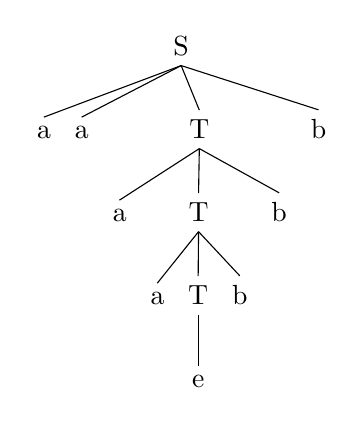
\begin{tikzpicture}
%    \Tree [.S [.aaTb [.aaaTbb [.aaaaTbbb [.aaaabbb ] ] ] ] ]
    \Tree [.S
              [.a ]
              [.a ]
              [.T
                  [.a ]
                  [.T
                      [.a ]
                      [.T
                          [.e ]
                      ]
                      [.b ]
                  ]
                  [.b ]
              ]
              [.b ]
          ]
\end{tikzpicture}

\subsection*{c.}i:

G is ambiguous. For example take the string $w=aaaaabbb$. We have $2$ different derivations: \\
$S\implies aaTb\implies aaaTbb\implies aaaSbb\implies aaaaaTbbb\implies aaaaabbb$ and\\
$S\implies aaTb\implies aaSb\implies aaaaTbb\implies aaaaabbb$. \\

Now define an unambiguous grammar $G_u = \{\{S, T, P, a, b\}, \{a, b\}, R, S\}$ for $L$, where
\begin{flalign*}
    R = & \{ S \rightarrow T,      & \\
        &    T \rightarrow aaTb,   & \\
        &    T \rightarrow aab,    & \\
        &    T \rightarrow aaKb,   & \\
        &    K \rightarrow P,      & \\
        &    P \rightarrow aPb,    & \\
        &    P \rightarrow ab   \} & \\
\end{flalign*}

Now try to prove $G_u$ is unambiguous.
Remember L = \{$w$ $|$ $w=a^ib^j$ and $2j\geq i\geq j > 0$\}.

\begin{enumerate}
    \item{\textit{Generating unequal number of a's and b's and the case of $i=2j$.}} \\
        We first use the rule $S\implies T$. After, if $i=2$ and $j=1$ then we directly use the rule $T\implies aab$. If $j>1$, then we can use the rule $T\implies aab$ only for termination of our string generating process. Before termination, we only use the rule $T\implies aaTb$ as we need. Note that in any step of string generation, we cannot use the rule $T\implies aaKb$ because if we use, we then have to use $K\implies P$ then have to use either $P\implies aPb$ or $P\implies ab$, which fails $i=2j$. There are no other possibilities. We have only one derivation.
    \item{\textit{Generating equal number of a's and b's. Not a real case, just will be used below.}} \\
        Suppose we somehow passed to $P$. If $i=1$ and $j=1$ then we directly use the rule $P\implies ab$. If $i>1$, then we use the rule $P\implies ab$ only for termination of our string generation process. Before termination, we only use the rule $P\implies aPb$ as we need. There are no other possibilities. We have only one derivation.
    \item{\textit{Case of $j<i<2j$.}}
        We first use the rule $S\implies T$. For such a string, we should do $k_1$ many $2\ a's-1\ b$ type generations, $k_1 - 1$ of them will be done before passing to $K$, and $k_2$ many $1\ a-1\ b$ type generations. According to $G_u$, in order to do $1\ a-1\ b$ type generatings, we should first use the rule $T\implies aaKb$, then the rule $K\implies P$ to be able to use the rules $P\implies aPb$ and $P \implies ab$. Note that this provides us to put (at least one time) unequal number of $a's$ and $b's$ to make $j>i$. Notice that if we pass to $P$, we cannot go back to $T$. Hence we should first do these $k_1 - 1$ generations, they can be done in only one way as stated in $(1)$, then use the rules $T\implies aaKb, K\implies P$ and after do those $k_2$ generations, again they can be done in only one way as stated in $(2)$. So, again, we have only one derivation for this case.
\end{enumerate}

Hence $G_u$ is unambiguous.

\section*{Answer 4}

$G = \{\{S, u, d, r, l\}, \{u, d, r, l\}, R, S\}$
\begin{flalign}
    R = & \{ S \rightarrow uSd,   & \\
        &    S \rightarrow rSl,   & \\
        &    S \rightarrow SS,    & \\
        &    S \rightarrow e   \} &
\end{flalign}

$S$ generates strings of length of an even number, which can be deriven easily from the set $R$. From the rule $(1)$ and $(2)$, we can derive that we can do an $u$ or $r$ movement at first, done at an odd numbered pass. After even number of moves, it is even due to $S$, we immediately do a $d$ (if an $u$ movement was done at the beginnig) or $l$ (if a $r$ movement was done at the beginning) movement, done at an even numbered pass. It also provides us that whehever we go up or right of a point, after doing a set of movements included in $S$, we go back by a $d$ or $l$ movement(accordingly), so we pass even number of times from a line segment.\\

From the rule $(4)$, we can derive that $e \in L$ and that whenever we satisfy the conditions $i$ and $ii$ given in the question, we can stop.\\

From the rule $(3)$, we can derive that whenever a set of movements included in $S$ is done, you can extend your path adding another $S$. This is because, in the first $S$, you already balanced your moves as desired in the question so you can do another set of $S$ movements, reminding us of the \textbf{concept of generating balanced parantheses}.


\section*{Answer 5}

\subsection*{a.}

$L=\{\ w\ |\ w=a^nb^n,\ n\geq 0 \}$

\subsection*{b.}

$L_1=\{\ w\ |\ w=a^ib^j,\ j\leq i\leq 2j,\ j>0\}$\\
$L_2=\{\ w\ |\ w=a^jb^i,\ j\leq i\leq 2j,\ j>0\}$\\
$L=L_1\cap L_2=\{\ w\ |\ w=a^ib^i,\ i>0\}$

\subsection*{c.}

$L_1=\{\ w\ |\ w=a^ib^ic^j,\ i,j\geq 0\}$\\
$L_2=\{\ w\ |\ w=a^jb^ic^i,\ i,j\geq 0\}$\\
$L=L_1\cap L_2=\{\ w\ |\ w=a^ib^ic^i,\ i\geq 0\}$

\section*{Answer 6}

\subsection*{a.}

Not a context free language. To prove that, use $Pumping\ Lemma\ for\ CFL$.\\
Choose $w = 0^{3^K}1^{K^2} = uvxyz\in L_1$ where $0 <|vy| \leq  K$. Now assume $L_1$ is a context free language. Then we should able to pump $v$ and $y$ as many times we want such that $w' = uv^ixy^iz\in L_1$. We have different cases for $v$ and $y$.

\begin{enumerate}
    \item{$v$ and $y$ are homogenous strings.}
        Say we pumped $v$ and $y$ only once such that $w'=uv^2xy^2z$. In that case, $v=0^{K-m}$ and $y=1^{m}$ where $K\geq m$ and $m$ depends on how we split $w$ into $uvxyz$ such that $v$ and $y$ are homogenous.\\
        Then $3^K + K^2 < |uv^2xy^2z| \leq 3^K + K^2 + K < 3^{K + 1} + (K + 1)^2$ so $w'\notin L_1$.
    \item{$v$ and $y$ are not homogenous strings.}
        That means either $v$ or $y$ is a string of $0s$ and $1s$ and the other one is empty string, a string of $0s$ or a string of $1s$ depending on the other string's position in $w$. Here the point, actually, is when one of $v$ or $y$ is a string of $0s$ and $1s$, then pumping this string fails the order of $0s$ and $1s$ so $w'\notin L_1$.
\end{enumerate}

\subsection*{b.}


$L_2 = L_{21} \cup L_{22}$ such that: $L_{21} = \{w\in \{a,b,c\}^* : n_a(w) \leq n_b(w)\}$ and $L_{22} = \{w\in \{a,b,c\}^* : n_a(w) > n_c(w)\}$. Since $L_{21}$ and $L_{22}$ are context free languages, then by the closure property of the context free languages $L_2$ is a context free language as well. Now first provide CFGs for $L_{21}$ and $L_{22}$.\\

$G_{21} = \{V_{21}, \{a, b, c\}, R_{21}, S_{21}\}$ where\\ \\
$V_{21}=\{S_{21}, T_{21}, a, b, c\}$
\begin{flalign*}
    R_{21} = & \{ S_{21} \rightarrow T_{21}T_{21},      & \\
                    &    T_{21} \rightarrow e,   & \\
                    &    T_{21} \rightarrow cT_{21},    & \\
                    &    T_{21} \rightarrow T_{21}c,   & \\
                    &    T_{21} \rightarrow T_{21}b,      & \\
                    &    T_{21} \rightarrow bT_{21},    & \\
                    &    T_{21} \rightarrow bT_{21}a,   \} & \\
                    &    T_{21} \rightarrow aT_{21}b,   \} & \\
\end{flalign*}

$G_{22} = \{V_{22}, \{a, b, c\}, R_{22}, S_{22}\}$ where\\ \\
$V_{22}=\{S_{22}, T_{22}, a, b, c\}$
\begin{flalign*}
    R_{22} = & \{ S_{22} \rightarrow T_{22}aT_{22},      & \\
                    &    T_{22} \rightarrow e,   & \\
                    &    T_{22} \rightarrow bT_{22},    & \\
                    &    T_{22} \rightarrow T_{22}b,   & \\
                    &    T_{22} \rightarrow T_{22}a,      & \\
                    &    T_{22} \rightarrow aT_{22},    & \\
                    &    T_{22} \rightarrow cT_{22}a,   \} & \\
                    &    T_{22} \rightarrow aT_{22}c,   \} & \\
\end{flalign*}

Hence  $G_{2} = \{V_{21}\cup V_{22}\cup \{S_2\}, \{a,b,c\}, R_{21}\cup R_{22}\cup \{S_2\rightarrow S_{21}, S_2\rightarrow S_{22}\}, S_2\}$.

\subsection*{c.}

Not a context free language. Say $L' = \{w | w=a^{10n}b^{6n}c^{15n}, n\geq 0\}$. Observe that $L' = L_3 \cap a^*b^*c^*$. If $L_3$ was a CFL then $L'$ would also be a CFL. However, since $L'$ is not a CFL then $L_3$ is not a CFL. Now prove $L'$ is not a CFL:

\begin{proof} Proof by pumping lemma.
    Choose $w = a^{10k}b^{6k}c^{15k} = uvxyz\in L_3$ where $0 <|vy| \leq  k$. Now assume $L_3$ is a context free language. Then we should able to pump $v$ and $y$ as many times we want such that $w' = uv^ixy^iz\in L'$. We have different cases for $v$ and $y$.\\

    First case. $v$ and $y$ includes all the letters a, b, c from alphabet such that either v or y includes two of the letters in an arbitraty length. In that case, as we pump the one including two letters of the alphabet fails the order of $as$, $bs$ and $cs$ so this case creates strings which do not belong to $L'$.\\ \\
    Second case. $v$ and $y$ do not include at least one of the letters from the alphabet such that either one or two of the letters cannot be pumped as we pump $v$ and $y$. Hence the string obtained by the pumping indicated in that case results in a string, not obeying the rule $10k-6k-15k$, in other words $w'\notin L'$. \\
    As a result,  $L'$ is not a CFL.
\end{proof}



\end{document}

​

